%%%%%%%%%%%%%%%%%%%%%%%%%%%%%%%%%%%%%%%%%
% Custom Class
% LaTeX Template
% Version 1.0 (28/2/15)
%
% This template has been downloaded from:
% http://www.LaTeXTemplates.com
%
% Original author:
% Vel (vel@latextemplates.com)
%
% License:
% CC BY-NC-SA 3.0 (http://creativecommons.org/licenses/by-nc-sa/3.0/)
%
%%%%%%%%%%%%%%%%%%%%%%%%%%%%%%%%%%%%%%%%%

%----------------------------------------------------------------------------------------
%	DOCUMENT SPECIFICATIONS
%----------------------------------------------------------------------------------------

% Class options are specified in the square brackets before the class name
% The example class has two custom options: OPONE or OPTWO; one of these MUST be used or the compilation fails
\documentclass[OPONE]{example}
\usepackage{amsmath}
\usepackage{amssymb}
\usepackage{commath}
\usepackage{graphicx}
\graphicspath{ {./} }
%----------------------------------------------------------------------------------------

\begin{document}

%----------------------------------------------------------------------------------------
%	DOCUMENT CONTENT
%----------------------------------------------------------------------------------------

\noindent Question 5 \\

Use the definition of $\Theta$ in order to show the following: \\

\begin{list}{}{}
	
	\item {\textbf{Definition:}} 
	
	Let f and g be two functions \textbf{$Z^{+}$} to \textbf{$Z^{+}$} \\ 
	$f = \Theta(g)$ if $f = O(g)$ and $f = \Omega(g)$. \\
	\\
	
	\begin{center}
		\line(1,0){250}
	\end{center}

	\item {a.}  
	$5n^{3} + 2n^{2} + 3n = \Theta(n^{3})$  \\
	\\
	\textbf{Proof that $f$ is $O(g)$} \\ 
	\\
	$f(n) = 5n^{3} + 2n^{2} + 3n$ \\
	$g(n) = n^{3}$ \\
	\\
	\textbf{Claim $f = O(g)$: }\\
	\\
	1. Select $c = 10$ and $n_{0} = 1$.  We will show that for any $n \geq 1$, $f(n) \leq 10g(n)$. \\
	2. Explicitly, $5n^{3} + 2n^{2} + 3n \leq 10n^{3}$.\\
	\\
	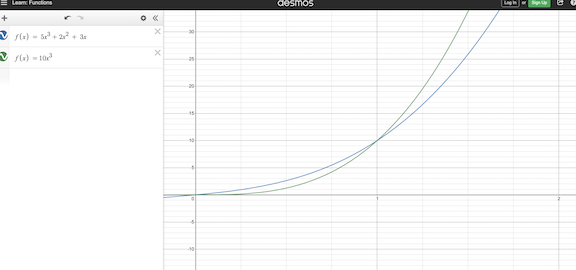
\includegraphics{grapha} \\ 
	\\
	\textbf{Facts:} \\
	1. Since $n \geq 1$, $n \leq n^{2} \leq n^{3}$.\\
	\\
	\textbf{Substitutions:} \\
	$f(n) = 5n^{3} + 2n^{2} + 3n$ \hspace{1.06 in} ...now given fact 1, substitute $n^{3}$ for both $n^{2}$ and $n$... \\
	$f(n)  \leq 5n^{3} + 2n^{3} + 3n^{3}$  \hspace{1 in} ...now adding factors of $n^{3}$ we obtain... \\
	$f(n) \leq 10n^{3}$ \hspace{1.682 in} ...add observing $g(n) = n^{3}$ we substitute and obtain... \\
	$f(n) \leq 10g(n)  \blacksquare$ \\
	
	\newpage 
	
	\textbf{Proof that $f$ is $\Omega(g)$} \\ 
	\\
	$f(n) = 5n^{3} + 2n^{2} + 3n$ \\
	$g(n) = n^{3}$ \\
	\\
	\textbf{Noting: }\\
	\\
	If $f(n)$ is a polynomial of degree $k$, then $f = \Omega(n^{k})$ only if the coefficient of the $n^{k}$ term in $f$ (call it $a_{k}$) is positive. Here are combinations for $c$ and $n_{0}$ that suffice as a witness to show that $f = \Omega(n^{k})$.
	
	If $f$ has no negative coefficients, then $c = a_{k}$ and $n_{0} = 1$ suffice.
	If $f$ has negative coefficients (but $a_{k} > 0$), then let $A$ be the sum of the absolute values of the negative coefficients in $f(n)$. The choices $c = a_{k}/2$ and $n_{0} = max\{1, 2A/(a_{k})\}$ are sufficient. \\
	\\
	\textbf{Claim $f = \Omega(g)$: }\\
	\\
	1. Noting the polynomial has all positive coefficients, $c = a_{k}$ and $n_{0} = 1$ will suffice. \\
	2. Select $c = 5$ and $n_{0} = 1$.  We will show that for any $n \geq 1$, $f(n) \geq 5g(n)$. \\
	2. Explicitly, $5n^{3} + 2n^{2} + 3n \geq 5n^{3}$.\\
	\\
	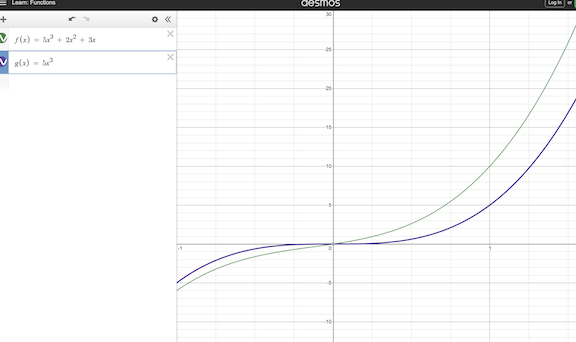
\includegraphics{grapha2} \\ 
	\\
	\textbf{Facts:} \\
	1. Since $n \geq 1$, $3n \geq 0$.\\
	2. Since $n \geq 1$, $2n^{2} \geq 0$.\\
	3. Since $n \geq 1$, $5n^{3} \geq 0$.\\
	\\
	\textbf{Building the inequality:} \\
	Starting with fact 1...\\
	$3n \geq 0$ \hspace{1.43 in} ...now using fact 2 add the inequalities to obtain...\\
	$2n^{2} + 3n \geq 0$ \hspace{1.1 in} ...now using fact 3, we can add $5n^{3}$ to both sides of the inequality...\\
	$5n^{3} + 3n^{2} + 3n \geq 5n^{3}$ \hspace{0.53 in} ...fact 3 also ensures sign of inequality does not change...\\
	\\
	Now observing $g(n) = n^{3}$  and $f(n) = 5n^{3} + 2n^{2} + 3n$ we substitute and obtain... \\
	$f(n) \geq 5g(n)  \blacksquare$ \\
	\\

\newpage

	\begin{center}
	\line(1,0){250}
\end{center}

	\item{b.}  
	$\sqrt{7n^{2} + 2n - 8} = O(n)$ \\
	
\textbf{Proof that $f$ is $O(g)$} \\ 
	\\
	$f(n) = \sqrt{7n^{2} + 2n - 8} $ \\
	$g(n) = n$ \\
	\\
	
\textbf{Claim $f = O(g)$: }\\
	\\
	1. Select $c = 3$ and $n_{0} = 1$.  We will show that for any $n \geq 1$, $f(n) \leq 3g(n)$. \\
	2. Explicitly, $\sqrt{7n^{2} + 2n - 8} \leq 3n$.\\
	\\
	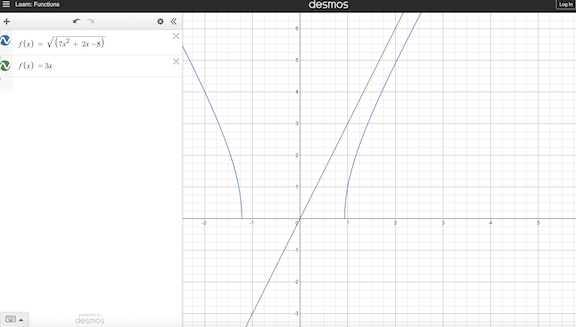
\includegraphics{graphb} \\ 
	\\
\textbf{Facts:} \\
	1. Since $n \geq 1$, $n \leq n^{2}$.\\
	2. $0 \geq -8$ \\
	3. Since $n^{2} \geq 1$, $9n^{2} - 8 \geq 1$ \\
	
\textbf{Substitutions:} \\
	$f(n) = \sqrt{7n^{2} + 2n - 8} $ \hspace{1.06 in} ...now given fact 1, substitute $n^{2}$ for $n$... \\
	$f(n)  \leq \sqrt{7n^{2} + 2n^{2} - 8} $  \hspace{1 in} ...now consolidating terms we obtain...\\
	$f(n) \leq \sqrt{9n^{2} - 8}$\hspace{1.42 in} ...now given fact 2 we obtain...\\
	$f(n) \leq \sqrt{9n^{2}}$ \hspace{1.62 in} ...and given fact 3, we can take square root to obtain... \\
	$f(n) \leq 3n$  \hspace{1.80 in} ...add observing $g(n) = 3n$ we substitute and obtain... \\
	$f(n) \leq 3g(n)  \blacksquare$ \\
	\\
	
\newpage
	
\textbf{Proof that $f$ is $\Omega(g)$} \\ 
\\
$f(n) = \sqrt{7n^{2} + 2n - 8} $ \\
$g(n) = n$ \\
\\
\textbf{Noting: }\\
\\
If $f(n)$ is a polynomial of degree $k$, then $f = \Omega(n^{k})$ only if the coefficient of the $n^{k}$ term in $f$ (call it $a_{k}$) is positive. Here are combinations for $c$ and $n_{0}$ that suffice as a witness to show that $f = \Omega(n^{k})$.

If $f$ has no negative coefficients, then $c = a_{k}$ and $n_{0} = 1$ suffice.
If $f$ has negative coefficients (but $a_{k} > 0$), then let $A$ be the sum of the absolute values of the negative coefficients in $f(n)$. The choices $c = a_{k}/2$ and $n_{0} = max\{1, 2A/(a_{k})\}$ are sufficient. \\
\\
\textbf{Claim $f = \Omega(g)$: }\\
\\
1. Given the presence of negative coefficients (but $a_{k} > 0$),  we calculate $A = \sqrt{\abs{-8}}$.\\
2. Additionally, $a_{k} = \sqrt{7}$. \\
3. As such, we select $c = \frac{\sqrt{7}}{2}$ and $n_{0} = max\{1, 
		\frac{
			2(\sqrt{8})
		}{
			\sqrt{7}
		}
\}$ which leaves us with $n_{0} = 
		\frac{
			2(\sqrt{8})
		}{
			\sqrt{7}
		}$
.  \\
4. We will show that for any $n \geq 
			\frac{
			2(\sqrt{8})
		}{
			\sqrt{7}
}$, $f(n) \geq \frac{\sqrt{7}}{2}g(n)$. \\
5. Explicitly, $ \sqrt{7n^{2} + 2n - 8}  \geq  \frac{\sqrt{7}}{2}n$.\\
\\
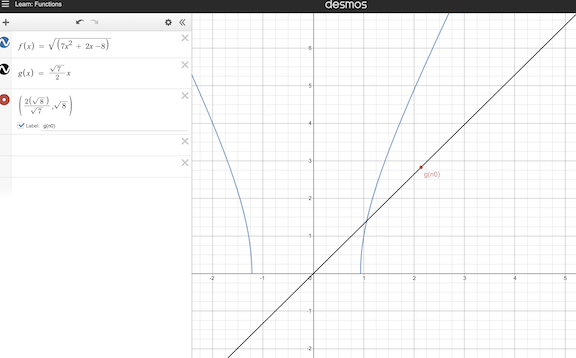
\includegraphics{graphb2} \\ 
\\
\\
\textbf{Building the inequality:} \\
$f(n) = \sqrt{7n^{2} + 2n - 8} $ \hspace{1.0 in} ...now factoring out $n^{2} $ we obtain...\\
$f(n) = \sqrt{n^{2}(7 + \frac{2}{n} - \frac{8}{n^{2}})} $ \hspace{.85 in} ...now we can take the $n^{2}$ out of root to obtain...\\
$f(n) = n\sqrt{7 + \frac{2}{n} - \frac{8}{n^{2}}} $ \hspace{1.05 in} ...knowing the limit of a sum is the sum of the limits...\\
$f(n) \geq \sqrt{7}n $ \hspace{1.65 in} ...as it will never obtain this value (asymptotic)...\\
$f(n) \geq \frac{\sqrt{7}n}{2} $ \hspace{1.65 in} ...and diving by a positive 2 maintains the inequality...\\
\\
Now observing $g(n) = n$  we substitute and obtain... \\
$f(n) \geq \frac{\sqrt{7}}{2}g(n)  \blacksquare$ \\
\\

\end{list}


%----------------------------------------------------------------------------------------

\end{document}